\level{2}{AAkkuSimu}

\level{3}{Structure}
{
\centering{}
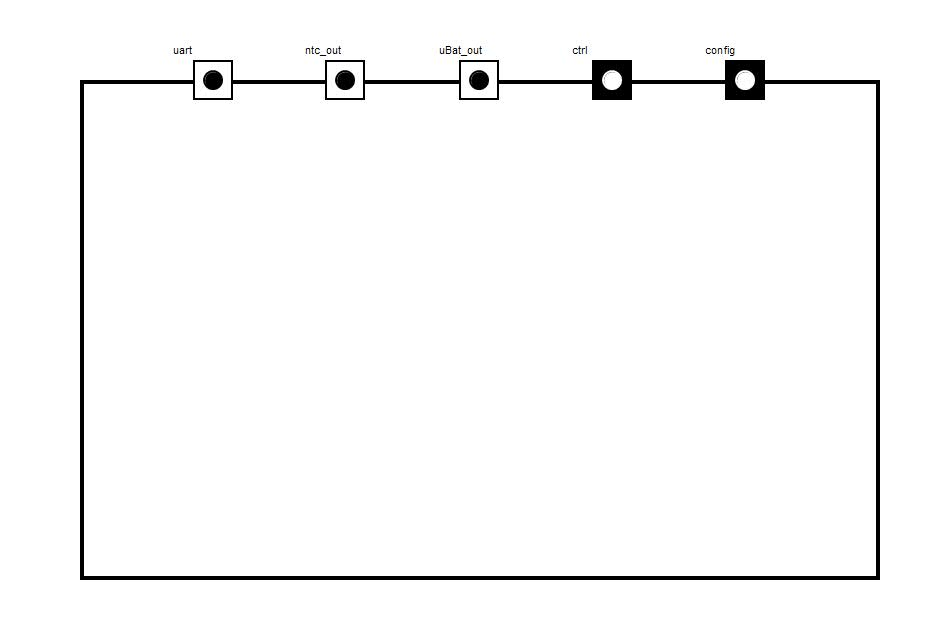
\includegraphics[width=1.0\textwidth]{./images/AAkkuSimu_structure.jpg}
\figcaption{AAkkuSimu Structure}
}

\level{3}{Ports}
\begin{tabular}[ht]{|l|l|l|l|l|p{5cm}|}
\hline
\textbf{Name} & \textbf{Protocol} & \textbf{Type} & \textbf{Kind} & \textbf{Multiplicity} & \textbf{Description}\\
\hline
uart & PAkkuSim & conj. & external & 1 & \\
\hline
ntc\_out & PDac & conj. & external & 1 & \\
\hline
uBat\_out & PDac & conj. & external & 1 & \\
\hline
ctrl & PAkkuCtrl & reg. & external & 1 & \\
\hline
config & PAkkuConfig & reg. & external & 1 & \\
\hline
\end{tabular}

\level{3}{Behavior}
\level{4}{Top Level}
{
\centering{}
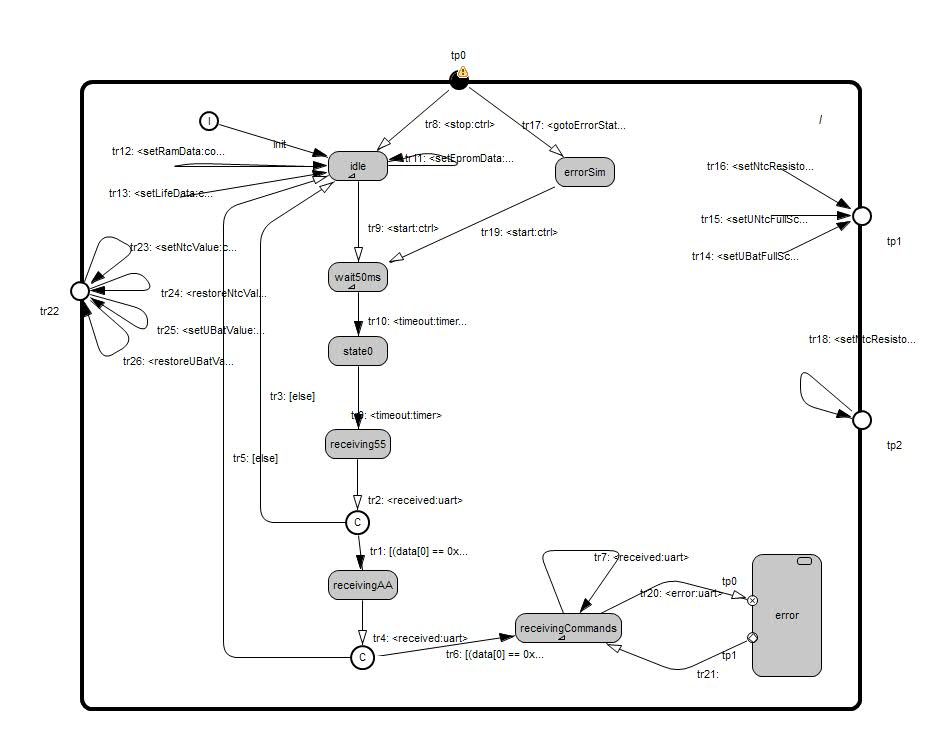
\includegraphics[width=1.0\textwidth]{./images/AAkkuSimu_behavior.jpg}
\figcaption{AAkkuSimu Top State}
}

\begin{par}

\end{par}

\level{4}{Subgraph error}
{
\centering{}
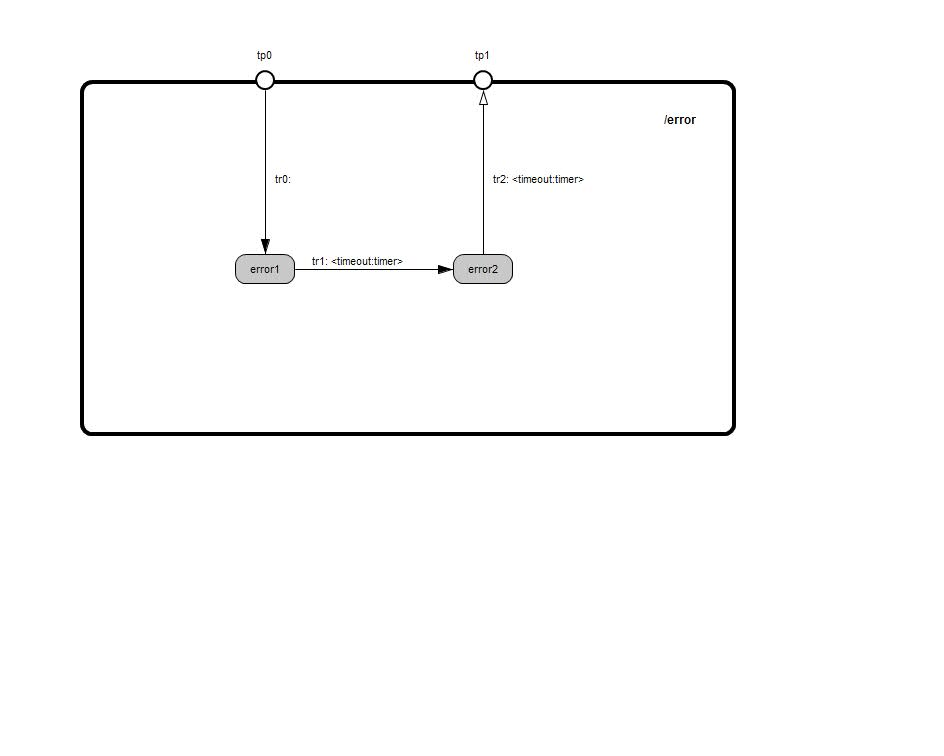
\includegraphics[width=1.0\textwidth]{./images/AAkkuSimu_error_behavior.jpg}
\figcaption{AAkkuSimu\_error}
}

\begin{par}

\end{par}
	

\level{3}{Attributes}
\begin{tabular}[ht]{|l|l|p{8cm}|}
\hline
\textbf{Name} & \textbf{Type} & \textbf{Description}\\
\hline
sData & DSerialFrame & \\
\hline
epromData & akkuEpromData & \\
\hline
ramData & akkuRamData & \\
\hline
liveData & akkuLiveData & \\
\hline
uBatFullScale & uint32 & % begin text from user Documentation
Fullscale value for UBat in mV for DGate Small
% end text from user Documentation
\\
\hline
ntcReferenceResistor & uint32 & % begin text from user Documentation
Reference resistor in Ohm
% end text from user Documentation
\\
\hline
ntcFullScale & uint32 & % begin text from user Documentation
Fullscale value for UNtc in mV
% end text from user Documentation
\\
\hline
\end{tabular}

\level{3}{Operations}
\begin{tabular}[ht]{|l|l|}
\hline		
	Name: & getNtcDacValFromTemp\\
	\hline
	ReturnType: &  uint32\\
	\hline
	Arguments: & temp:int8\\
	\hline
\end{tabular}
\newline\newline\newline
\begin{tabular}[ht]{|l|l|}
\hline		
	Name: & getUBatDacValFromVoltage\\
	\hline
	ReturnType: &  uint32\\
	\hline
	Arguments: & voltage:int32\\
	\hline
\end{tabular}
\newline\newline\newline
